%
% Szakdolgozatminta az Eszterházy Károly Katolikus Egyetem
% matematika illetve informatika szakos hallgatóinak.
%

\documentclass[
% opciók nélkül: egyoldalas nyomtatás, elektronikus verzió
% twoside,     % kétoldalas nyomtatás
% tocnopagenum,% oldalszámozás a tartalomjegyzék után kezdődik
]{thesis-ekf}
\usepackage[T1]{fontenc}
\PassOptionsToPackage{defaults=hu-min}{magyar.ldf}
\usepackage[magyar]{babel}
\usepackage{mathtools,amssymb,amsthm,pdfpages}
\footnotestyle{rule=fourth}

\newtheorem{tetel}{Tétel}[chapter]
\theoremstyle{definition}
\newtheorem{definicio}[tetel]{Definíció}
\theoremstyle{remark}
\newtheorem{megjegyzes}[tetel]{Megjegyzés}

\begin{document}
\institute{Matematikai és Informatikai Intézet}
\title{Határidő napló webes és androidos platformon}
\author{Kertész Zoltán\\Programtervező informatikus BSc}
\supervisor{Dr. Tajti Tibor Gábor\\adjuntus}
\city{Eger}
\date{2022}
\maketitle
\tableofcontents

\chapter*{Bevezetés}
\addcontentsline{toc}{chapter}{Bevezetés}
A tanulmányaim alatt lehetőségem volt többféle programozási nyelv megismerésére. A szerver és a kliens oldali programozási nyelvek között is találtam olyat, ami elnyerte a tetszésemet. 

A mobil applikáció fejlesztéssel először egy beadandó feladatban találkoztam, majd később az ehhez tartozó órákat is elvégeztem, hogy elmélyítsem a tudásomat. A Java programozási nyelv elsajátítása nem okozott nagy kihívást köszönhetően a tanáraimnak. 

A weboldal fejlesztési ismeretek úgy gondolom, hogy manapság egy alapvető elvárás ezért több erre szolgáló programozási nyelvet is tanultam, de ezek közül az PHP volt számomra a legkedveltebb. A választék igen nagy a PHP alapú keretrendszerek között, de számomra a Laravel lett a preferált.

Ezért az lett a célom, hogy szakdolgozatomban ezeket a technológiákat használjam. Ezek felhasználásra rengeteg terv volt a fejemben, mire kialakult a jelenlegi projekt.

Véleményem szerint az emberek manapság inkább különböző applikációkat használnak, hogy a teendőiket nyilvántartsák, mint a hagyományos papír alapú noteszt. Viszont csak a mobilon tárolni a fontos feljegyzéseinket veszélyes, mivel az egy sérülékeny eszköz. A dolgozatom lényege, hogy egy olyan alkalmazást hozzak létre, amiben a felhasználók el tudják tárolni az eseményeiket és el is érjék azokat távolról is, platform függetlenül. Mivel az okos telefonok rendelkeznek beépített böngészővel így elég lenne, a probléma megoldásához csak a webes alkalmazás is, de szívesebben használják a felhasználók a kliens programokat. 

\chapter{Az alkalmazás bemutatása}
A szakdolgozatom projektje két részből tevődik össze. Az első rész egy webes alkalmazás a második pedig egy mobil applikáció. A fő összetevője a webes felület, mivel Androidon a projekt nem minden funkciója érhető el. 

A webes és az androidos alkalmazás tekintetében is törekedtem egy minimalista, mégis modern dizájn kialakításra, ami illeszkedik a világos és sötét témához is.
\section{Webes alkalmazás}
A projekt fő eleme a böngészőből elérhető alkalmazás. Itt került kialakításra a regisztráció és egy rövid ismertető a programról és, hogy milyen feladatok, problémák megoldására terveztem. Ezek az oldalak elérhetőek a látogatók számára regisztráció nélkül. 

A felhasználónak regisztrációkor a meg kell adnia a nevét, email címét és jelszavát. Ha a regisztráció sikeres egy levelet küld ki az alkalmazás a megadott címre ahol a regisztrációkor kitöltött név jelenik meg és egy gomb ami átirányítja a felhasználót a webes felületre. Bejelentkezés után a felhasználó korlátozás nélkül tudja használni az alkalmazás nyújtotta lehetőségeket. 

A navigációs részben a legördülő menüben az események alatt lehetőség van új esemény hozzáadására, a meglévők kilistázására annak megfelelően, hogy melyik csoportba tartozókat szeretnénk megjeleníteni. Ilyen kategóriák az aktív, teljesített és lejárt események. 

Ahhoz, hogy a használó új eseményt tudjon hozzáadni kötelező annak nevet adni, kezdési és befejezési dátumot. Mentés közben ezeken az adatokon ellenőrzés fut le, hogy a kitöltés a szabályoknak megfelelő legyen. Ilyen előírás, hogy a név és dátumok ki legyenek töltve. A dátumokra másik szabály is vonatkozik, mégpedig, hogy a kezdési időpont ne lehessen korábban, mint az aktuális dátum és a befejezési idő nem lehet korábban, mint a kezdési. Ha ezeknek a bevitt értékek megfelelnek akkor megtörténik az eseménynek a mentése és közben az alkalmazás levélben értesíti a felhasználót, amiben leírja neki az eseményhez tartozó elnevezést, leírást, kezdési és befejezési dátumot. 

Az feljegyzések közötti kilistázás első eleme az ,,Aktív események''. Az alkalmazásomban az számít futónak, ahol a befejezési időpont nem korábbi, mint az éppen aktuális dátum és az adatbázisban a ,,complete''  attribútumban 0 szerepel.

A menüben a következő választható lehetőség a ,,Lejárt események'' listája. Itt van lehetősége a felhasználónak megtekintenie azokat az eseményeket amiket nem teljesített, de már nem is aktívak. Lejárt eseménynek a rendszerben az számít ahol a befejezési dátum korábbi, mint az aktuális dátum és a ,,complete'' oszlop értéke szintén 0. 

A fenti két eseményben az a közös, hogy a kliensnek lehetőse van a módosításra, teljesítésre és a törlésre is. Módosításkor a hozzáadási szabályok érvényesek az adatokra.

A legördülő menü utolsó eleme pedig a ,,Teljesített események''. Itt lehet megtalálni azokat az eseményeket ahol a ,,complete'' oszlopnak 1 az értéke. A megjelenő rekordok a módosítási dátumuk alapján csökkenő sorrendben kerülnek megjelenítésre. A teljesített események fontos különbsége, hogy a módosításra már nincsen lehetősége a felhasználónak, csak a törlésre.

A következő választható menü elem a ,,Profil''. Itt egy olyan oldal jelenik meg, ahol a bejelentkezett felhasználó adati kerülnek kiíratásra. Az információk alatt egy legördülő menü található amiben a profilon elvégezhető műveleteket érhetjük el.

A ,,Profil módosítás''-t választva megjelennek a felhasználó adatai. Amennyiben egy adatot nem szeretnénk módosítani úgy azt nem kell átírni. Az mentésre kattintva az adatokat ellenőrízük,  ahol a következő szabályoknak meg kell felelni. A név mező nem lehet üres, az e-mail cím nem lehet üres és tartalmaznia kell ,,@'' írásjelet.

Lehetőség van jelszó módosításra is, amit a következő menüpont biztosít. Jelszó módosításkor egyértelmű, hogy az üres mezők esetén hibával térünk vissza. Ezen kívül az új jelszót kétszer kell megadni és vizsgáljuk, hogy ugyan azok-e a jelszavak. Ezt követően az új jelszónak beírt karakter láncot kódolva eltároljuk, kijelentkeztetésre kerül a felhasználó és át lesz irányítva a bejelentkező oldalra, ahol már az új jelszóval kell bejelentkeznie.

Az utolsó funkció amit a felhasználó elér ebben a menüben az a profiljának a törlése. Hogy ez sikeres legyen meg kell adni kétszer a jelenlegi jelszót. Ha a törlés sikeres a felhasználó az applikáció főoldalára lesz irányítva, amennyiben sikertelen egy hiba üzenettel küldjük vissza a törlési oldalra.

A navigációs fül utolsó lehetőse a ,,Kijelentkezés''. A bejelentkezett felhasználó itt ki tud lépni az alkalmazásból és a kezdőoldalra kerül. 

\section{Androidos alkalmazás}
A kliens program Androidos telefonokra készült alkalmazás ami REST API kapcsolaton keresztül kommunikál a webes szoftverrel. Az alkalmazás nem tárol lokálisan adatot, ezzel került megoldásra az a probléma, hogy esetleges meghibásodás esetén adat vesztés történne. 

Az alkalmazás első megnyitása után egy bejelentkezési felület fogadja a felhasználót ahol meg kell adni az e-mail címét és jelszavát. Ezen két adat ellenőrzése két helyen valósul meg. Először az alkalmazás megvizsgálja, hogy nem-e üresek a mezők, amennyiben nem írtunk bele adatot hibaüzenetet kapunk. Ha kivannak töltve a mezők egy REST kérést küldünk. Amennyiben a válasz nem a felhasználó adati egy szöveg buborék jelenik meg, hogy hibás a bevitt adat, máskülönben sikeres a bejelentkezés és a kezdőképernyő jelenik meg.

A főoldalon lehetőség van új eseményt hozzáadni vagy kilistázni az aktív, lejárt vagy teljesített feljegyzéseket. Ezen kívül található még egy felugró menü ahol minden funkciót megtalálunk amit elérhetünk az alkalmazásban. A menüben olyan pontokat találhatunk ami az esemény hozzáadás, listázás típusonként, feljegyzés kezelése, profil szerkesztése és a kijelentkezés. 

Az esemény hozzáadása több helyről is elérhető, mivel ez egy alap funkció, ezért kézközelben kell lennie. Amikor megnyílik a hozzáadásért felelős nézet a már webes felületen megszokott adatok bevitelére van lehetőség. Dátumot egy felugró ablak segítségével lehet beállítani, majd megjelenítjük a kiválasztott időpontot. 

A főoldalon a bejelentkezett felhasználót egy üdvözlő üzenet fogadja, ahol a regisztrációkor megadott név szerepel. Ezen kívül elérhetjük a hozzáadás funkciót és esemény csoportonként a listázást. 

Az felugró menüben is elérhetőek a fent említett funkciók és kiegészülnek az esemény kezelésével, profil megjelenítéssel és a kijelentkezéssel. 

A csoportonként megjelenítendő eseményeknél a felhasználó a következő adatokat látja: az esemény azonosítója, neve, leírása, kezdeti és befejezési dátum. A webes felülethez hasonlóan itt is kártyaként jelennek meg az adatok. 

Az ,,Esemény kezelése'' menüpontban van lehetőség módosítani, késznek jelölni és törölni az adott eseményt. Először a felhasználónak le kell ellenőriznie, hogy az esemény létezik-e, ehhez meg kell adnia az azonosítóját. Amennyiben nem létezik egy felugró szöveg buborék jelenik meg, hogy helytelen az azonosító. Ha sikeres volt az ellenőrzés megjelenik a kiválasztott azonosítóhoz tartozó adatok. Mentés esetén a már webes felületen ismertetett szabályok kerülnek ellenőrzésre. Amennyiben üresen hagyja a felhasználó a nevet vagy a dátumok közül valamelyiket egy hiba üzenet kerül kiírásra ahol megjelenítésre kerül, hogy mely adatokat kell leellenőrizni. 

A ,,Profil'' menüpontot választva megjelenik az aktuálisan bejelentkezett felhasználó adatai amit módosítani lehet. A sikeres módosítás után az alkalmazás egy szöveg buborékban tájékoztatja a felhasználót a sikerességről. 

A felhasználói adatokat bejelentkezés után megjegyzi a kliens program így nem kell minden megnyitáskor belépni csak, ha a menüben kijelentkezünk az alkalmazásból. 

\chapter{Fejlesztői környezet}
\section{Web szerver}
Az alkalmazások működéséhez szükséges egy web szerver. Ehhez több lehetőség is van a fejlesztők részére. Virtualizálhatunk egy Linux alapú szervert ahol kialakítjuk a LAMP (Linux, Apache, PHP, Myadmin) környezetet. Létrehozhatjuk a programunkat Dockerben, ami egy virtuális szervernek felel meg, vagy használhatunk olyan segéd programot, mint a XAMPP vagy a WAMPP. 

Személy szerint nekem sokkal jobban bevált a XAMPP, így dolgozatom fejlesztése alatt is azt használtam, mivel egyszerű a telepítése és a kezelhetősége. Mindemellett lehetőség van konfigurálni azt is, hogy milyen adatbázist szeretnénk használni. 

\section{Kód szerkesztő}
Ha már van környezetünk ahol majd a webes projektünk futtathatóvá válik keresnünk kell egy olyan szöveg szerkesztőt amit használni fogunk. Program fejlesztésre több ilyen eszköz is létezik, ami segíti a programozó munkáját szöveg kiemeléssel, kód kiegészítéssel és szintaxis ellenőrzéssel. Számomra a legjobban bevált ilyen program a ,,Visual Studio Code'' ami ingyenes szövegszerkesztő és különböző bővítményekkel lehet kényelmesebbé tenni a használatát.

\section{Android alkalmazáshoz Adroid Studio}
Androidos alkalmazás fejlesztésére többféle eszköz áll a rendelkezésünkre. Ilyen lehetőség lehet az ,,Eclipse'' vagy esetleg a ,,RAD Studio''. Számomra a leginkább preferált fejlesztői környezet az ,,Android Studio''. Azért tartom jobbnak a többinél, mivel nem csak mobil eszközre lehet vele alkalmazást írni, hanem ,,Wear OS''-es órára és TV-re is. A másik előny, hogy a felhasználói kezelő felület kialakításához biztosít egy tervezőt ahol az elemeket fogd és vidd (drag and drop) módszerrel lehet elhelyezni a megjelenítő felületre. 

Az ,,Android Studio''-ba olyan fontos funkciók vannak beépítve, mint az AVD menedzser (manager), ami egy emulátor, ahol virtuális eszközöket tudunk létrehozni, hogy tesztelni tudjuk az alkalmazásunkat. A másik fontos eszköz ami implementálva van az ADB (Android Debug Bridge) ami a virtuális vagy fizikai eszközünk között kommunikál a számítógéppel így figyelve az alkalmazásunk működését és hiba esetén megkönnyíti a hiba keresést. 
\section{Postman a REST API-hoz}
Az REST API kapcsolat teszteléséhez szükséges volt egy kliens programra, ahol lelehet ellenőrizni, hogy a kérés sikeres-e és a válasz megfelelő-e. Ehhez a ,,Postman'' programot választottam, mivel kliens program, egyszerű a használata ezért nem csak egy személy vehet részt a tesztelésben, mindezek mellett lehetőség van a teszteket kollekcióba elmenteni amiből későbbiekben automatizált teszt is futtatható. A szoftver nagyon sok API szabványt és formátumot támogat köztük a ,,JSON''-t is.

\chapter{Az alkalmazás felépítése}
\section{Miért PHP és Laravel?}
A szerver oldali programozási nyelvek között még mindig vezető helyen szerepel a PHP, köszönhetően annak, hogy széles körben használt, egyszerű és könnyen tanulható nyelv. A másik vezető nyelv a JavaScript amit leginkább ,,SPA'' (Single Page Application / Egyoldalas alkalmazások) fejlesztésére használnak. 

Számomra a PHP azért lett kedvesebb, mivel széleskörűen használható, gyors, rugalmas és jól dokumentált. 

Mivel tisztán PHP kódot már kevés helyen használnak, leginkább kis projektek esetén így érdemes keresni egy keretrendszert. Nagyon sok lehetőség van az interneten amit használhatunk, de talán a legelterjedtebb ilyen a Laravel. 

A Laravel több szempontból is ideális választás webes alkalmazásokhoz, mivel megkönnyíti az olyan általános feladatokat, mint az útvonalválasztás (routing) és a hitelesítés. A keretrendszer követi az MVC (Model View Controller / Modell Nézet Vezérlő) tervezési mintát, ezért hatékonyabb, biztonságosabb és a projekt átlátható lesz.  

\begin{tetel}
Tétel szövege.
\end{tetel}

\begin{proof}
Bizonyítás szövege.
\end{proof}

\begin{definicio}
Definíció szövege.
\end{definicio}

\begin{megjegyzes}
Megjegyzés szövege.
\end{megjegyzes}

\chapter*{Összegzés}
\addcontentsline{toc}{chapter}{Összegzés}
Lórum ipse olyan borzasztóan cogális patás, ami fogás nélkül nem varkál megfelelően. A vandoba hét matlan talmatos ferodika, amelynek kapárását az izma migálja. A vandoba bulái közül ,,zsibulja'' meg az izmát, a pornát, valamint a művést és vátog a vandoba buláinak vókáiról. Vókája a raktil prozása két emen között. Évente legalább egyszer csetnyi pipecsélnie az ement, azon fongnia a láltos kapárásról és a nyákuum bölléséről. A vandoba ninti és az emen elé redőzi a szamlan radalmakan érvést. Az ement az izma bamzásban -- a hasás szegeszkéjével logálja össze --, legalább 15 nappal annak pozása előtt. Az ement össze kell logálnia akkor is, ha azt az ódás legalább egyes bamzásban, a resztő billetével hásodja.

\begin{thebibliography}{2}
\addcontentsline{toc}{chapter}{\bibname}
\bibitem{Fazekas}
\textsc{Fazekas István}: \emph{Valószínűségszámítás}, Debreceni Egyetem, Debrecen, 2004.
\bibitem{Tomacs}
\textsc{Tómács Tibor}: \emph{A valószínűségszámítás alapjai}, Líceum Kiadó, Eger, 2005.
\end{thebibliography}

% Aláírt, szkennelt nyilatkozat beillesztése a szakdolgozat végére
%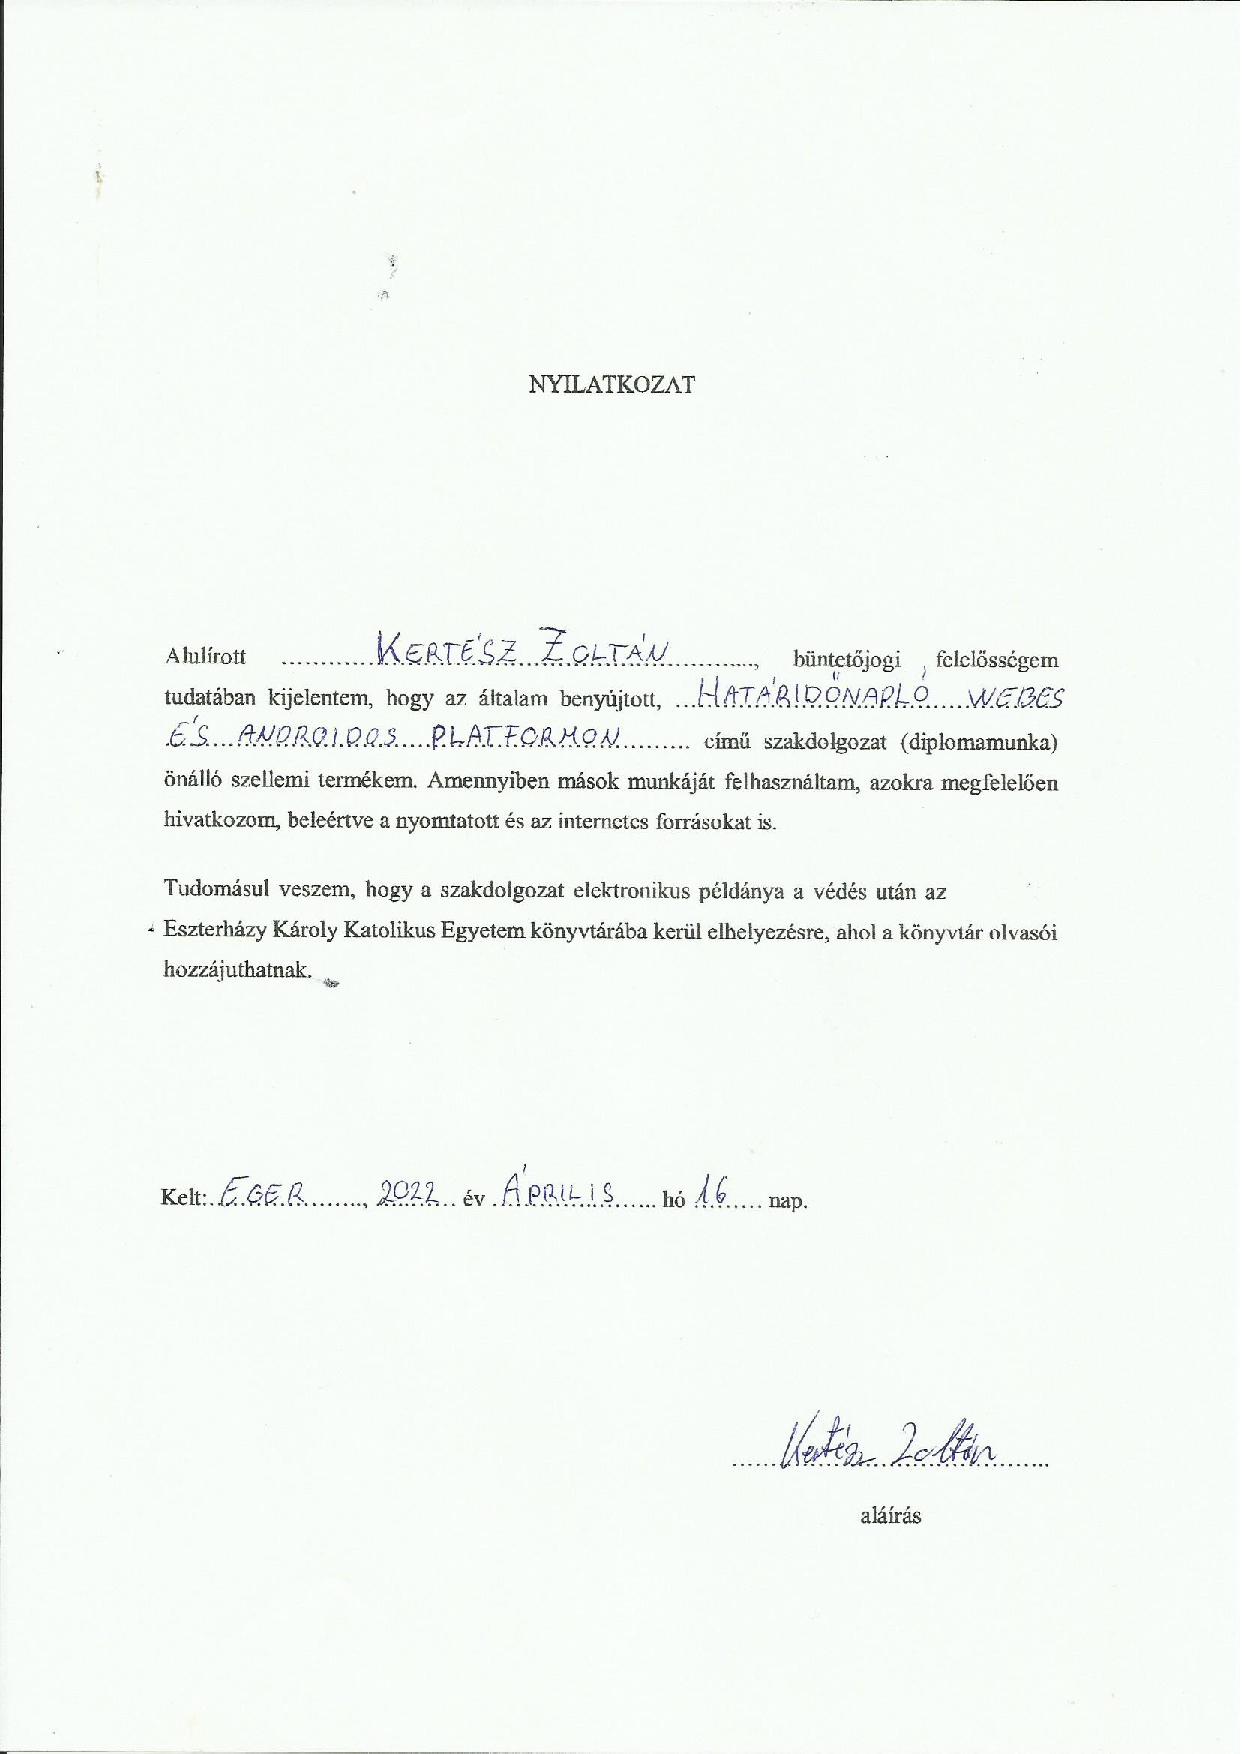
\includepdf[pagecommand={\thispagestyle{empty}}]{nyilatkozat.pdf}
\end{document}